\newcommand{\CLASSINPUToutersidemargin}{1.5in}
\documentclass[10pt,final,journal]{IEEEtran}
\usepackage{graphicx}
\usepackage{algorithm2e}
\usepackage{listings}

\begin{document}
\title{Troups: Scalable Transactions for BigTable datastores}
\author{Benjamin Busjaeger, Jonathan Chu, Daniel Ormond \\
\{busjaeg2, jmchu2, ormond1\}@illinois.edu}
\date{Feb 2012}
\maketitle

\begin{abstract}
Troups is a novel transaction manager for cloud datastores of the BigTable family that provides full ACID transactions across co-located data items. It includes a mechanism for grouping related rows and an algorithm that aids users in deciding what groups to form by identifying data types and items frequently accessed together in transaction logs. This allows us to improve the consistency guarantees of these systems without significantly impacting their high scalability or availability.
\end{abstract}

\begin{IEEEkeywords}
cloud, data storage, BigTable, transaction processing
\end{IEEEkeywords}

\section{Introduction}
Cloud platforms like Google and Amazon store vast amounts of data. This is in part because they pool resources to efficiently serve multiple tenants and in part because the volume of data produced by applications and users has significantly increased in recent years. At the same time users expect their data to always be quickly accessible anywhere and they have little tolerance for data loss or inconsistencies. Studies like ~\cite{Ramsay:1998} have shown that users quickly become  irritated by long response times and take their business elsewhere. Unfortunately, per Brewer's conjecture ~\cite{gilbert2002brewer}, it is not possible to maximize all of these goals simultaneously. These challenges have forced a change in the way data is stored and processed in the cloud.

Traditional relational database management systems (RDBMSs) are designed to provide high consistency by giving users the impression of a single system image. The conventional approach of improving availability and performance of these systems by purchasing more powerful and resilient hardware has obvious scalability limitations and is often not cost effective. The alternative of clustering traditional RDBMSs across less expensive hardware has its own set of challenges, since the single system objective implies high overhead from frequent distributed transactions and limited partition tolerance. Popular open source databases like MySQL have been shown to only scale to a small number of nodes ~\cite{Malkowski:2010:EAD:1774088.1774449} and commercial RDBMSs have similar limitations ~\cite{Campbell:2010:ESF:1807167.1807280}.

In response to the lack of scalability and high operational cost of traditional RDBMSs, large Internet companies have recently developed their own data storage solutions. Some notable examples of these so called NoSQL datastores are Google's BigTable ~\cite{Chang:2006:BDS:1267308.1267323}, Yahoo's PNUTS ~\cite{Cooper:2008:PYH:1454159.1454167}, and Amazon's Dynamo ~\cite{DeCandia:2007:DAH:1323293.1294281}. These architectures are radical departures from traditional RDBMSs in that they do not expose complex query operations and provide only limited consistency guarantees. This allows them to more efficiently partition data across dynamically scalable clusters and to isolate faults to subsets of the system.

Many cloud applications, like search index construction, can easily tolerate relaxed consistency guarantees. However, other applications, like emerging OLTP multi-tenant platforms, have strong isolation and atomicity requirements. Without sufficient transaction support built into the infrastructure, the burden of ensuring data integrity is ultimately placed on application developers.

Troups, which stands for Transaction Groups, aims to improve the transactional capabilities of NoSQL datastores in the BigTable family without compromising their scalability. To this end, it extends the BigTable programming model with the ability to group related rows in order to co-locate their data for efficient transaction processing. Troups also supports cross-group transactions, but tries to minimize their use to avoid two-phase commit overhead. Our transaction manager is novel in that it is designed as an observer, which means it extends BigTable without requiring changes and it is theoretically portable across datastores that satisfy the constraint model. We have also developed a set of group detection and placement algorithms to facilitate and optimize the task of identifying groups and allocating them to servers. In summary, our main contributions to the research field are:

\begin{enumerate}
\item A novel transaction manager for BigTable-like datastores that enables full ACID transactions at large scale for applications that exhibit transaction locality.
\item A set of group detection and Time Swap placement algorithms based on transaction logs.
\end{enumerate}

\section{Related Work}
Research on cloud-scale OLTP systems generally falls into two categories. On one hand, numerous approaches have been proposed recently for extending cloud datastores with more powerful transaction models. On the other hand, several recent publications describe how to adapt RDBMSs to make them more suitable for cloud workloads. The common theme across these approaches is a departure from full featured ACID transactions across the full data set. The proposals either reduce transaction isolation levels to make global transactions feasible or restrict serializable transactions to a subset of the data. In the latter case selection of these subsets is critical for ensuring efficient transaction processing, so algorithms have emerged to automate this process. We will first examine and classify OLTP cloud datastore architectures and subsequently survey relevant work on optimized data partitioning.

\subsection{OLTP Cloud Datastores}
\emph{Cloud SQL Server} ~\cite{Campbell:2010:ESF:1807167.1807280, Bernstein:2011:AMS:2004686.2005651}, \emph{ElasTraS} ~\cite{Das:2009:EET:1855533.1855540, Das:2010:EAE}, and \emph{Relational Cloud} ~\cite{Curino:2011:JPMWMBZ11} describe approaches for horizontally scaling out different relational DBMSs. Cloud SQL Server augments Microsoft SQL Server with partitioning and primary-copy replication. Serializable ACID transactions are supported, but limited to a single partition, which can be a whole logical database, referred to as a table group, or a set of rows from a table group that have been assigned a common partitioning key by the user. ElasTraS uses hierarchical schema-level partitioning and also restricts transactions to one partition. It differs from Cloud SQL Server in that it decouples storage from metadata management through the use of a distributed file system. This allows for a dynamic mapping between partitions and nodes. Relational Cloud combines a workload-aware approach for efficient data placement with a graph-based partitioning algorithm for data co-location discussed in the next section. ACID transactions are supported within and across partitions. Although our approach is not targeted at RDBMSs, it uses similar partitioning techniques.

\emph{Percolator} ~\cite{Peng:2010:LIP:1924943.1924961}, \emph{HBaseSI} ~\cite{Zhang:2010:5697970} and \emph{ReTSO} ~\cite{Junqueira:2011:LTS:2056318.2057148} are different approaches for adding global transactions with snapshot isolation \footnote{See Background section for details on snapshot isolation} semantics to BigTable-like datastores. Percolator is specifically designed to allow incremental search index construction, so it is optimized for throughput and not suitable for latency-sensitive applications. HBaseSI is a pure client API that uses a set of custom tables and atomic test-and-set operations to manage transactions without central coordination. ReTSO implements a lock-free commit algorithm using a centralized Transaction Status Oracle. The benefit of these approaches is that they do not rely on data co-location to support one-phase commit transactions. The downside is weaker isolation. Troups does not rely on a centralized concurrency control component, so it can offer stronger isolation, but it is less suitable for transactions that span any data in the cluster. Nevertheless, our approach adopts several ideas presented in ReTSO to implement efficient and non-invasive concurrency control.

\emph{G-Store} ~\cite{Das:2010:GSD:1807128.1807157} and \emph{CloudTPS} ~\cite{Wei:2011:5740834} build transaction capabilities targeted at specific use cases on top of BigTable-like datastores. G-Store introduces a key group protocol to provide ACID transactions over dynamically selected key sets. It is intended for applications which need to execute transactions across frequently changing groups of entities, that are non-overlapping, so it has limited applicability. CloudTPS is designed for web application workloads and assumes short-lived transactions that access small data sets known prior to starting the transaction. It interposes a group of Local Transaction Managers (LTMs) between clients and datastores which load data items and transaction state into memory for efficient processing. This implies the need for a separate server cluster with its own fail-over and recovery mechanisms.

\emph{MegaStore} ~\cite{Furman:2008:8530095, Baker:2011:8530095} tries to bridge the gap between RDBMSs and NoSQL datastores by augmenting BigTable with a declarative schema language. It provides strong consistency guarantees within fine-grained partitions, called entity groups, and ensures high availability by synchronously replicating mutations across datacenters. Troups is closely related to Megastore's transaction manager, but differs in several ways. In Megastore groups are the units of concurrency control and logging to enable wide-area network replication. Mutations are first appended to the replicated log and then applied to the datastore after commit. Reads within groups block until changes are applied, whereas reads across groups may not see the latest committed data. In Troups the unit of concurrency control is a cell and the log is tablet-scoped. This enables a high degree of concurrency and batch commit optimizations across groups. Mutations are directly written into the datastore and filtered for read operations. Therefore, readers can see the last written mutation, even if it has not been committed yet. The approaches also differ in how groups are defined, in Megastore entity groups are statically declared in the schema, whereas in Troups groups are dynamically formed based on programmatic grouping policies.

\emph{Deuteronomy} ~\cite{Levandoski:2011:8530161} is noteworthy, because it aims to decouple transaction management from the underlying datastore, a goal shared by our approach. To this end, it defines a transaction component (TC) capable of providing full ACID transactions for any datastore that implements a well-defined data component (DC) interface. The TC applies concurrency control and undo/redo logging at the logical record level as opposed to at the physical page level. Our transaction manager also operates against an abstract datastore contract. Our approach differs from Deuteronomy in that it uses different concurrency control and recovery algorithms and does not rely on a centralized transaction manager.

Table ~\ref{classification} summarizes the classification discussed above.

\begin{table}[!t]
\renewcommand{\arraystretch}{1.3}
\caption{OLTP Cloud Data Store Classification}
\label{classification}
\centering
\begin{tabular}{|c|c|c|c|}
\hline
\bfseries Data Store  & \bfseries Data Model & \bfseries  Part. & \bfseries Isolation \\
\hline
\hline
Cloud SQL & relational & yes & serializable \\
ElasTraS & relational & yes & serializable \\
Rel. Cloud & relational & yes & serializable \\
Percolator & BigTable & no & snapshot \\
HBaseSI & BigTable & no & snapshot \\
ReTSO & BigTable & no & snapshot \\
G-Store & BigTable & yes & serializable \\
CloudTPS & BigTable & no & serializable \\
Megastore & BigTable & yes & serializable \\
Deuteronomy & agnostic & no &serializable \\

\hline
\end{tabular}
\end{table}

\subsection{Paritioning Algorithms}
There are multiple partitioning algorithms in use and in study currently.  Not all of the algorithms have the same goal.  Hash-based algorithms help scale the database by evenly distributing the data on different nodes while other algorithms have a more specific goal to reduce transaction overhead.

Schism ~\cite{Curino:2010:SWA:1920841.1920853} is a static partitioning algorithm to reduce distributed transactions for SQL datastores. It uses transaction logs to determine how to partition data. The transaction anaylsis is similar to the work done by Chun-Hung et al.~\cite{chun:2002} It significantly improves performance compared to hash-based and even manual partitioning techniques. These static algorithms are a good starting point for our work and would likely yield better results for key/value stores given their simplified data access model. Also, an incremental version of these algorithms may scale better than the static equivalent, since it may be able to consider only new transaction log entries in each iteration. Another option would be to use a probabilistic algorithm.

Hehme and Bruno ~\cite{Nehme:2011:APD:1989323.1989444} present and algorithm that deeply integrates directly with the parallel query optimizer in Microsoft SQL Server.  Their algorithm provides a static data partitioning recommendation.  Their goals was to provide a data partition strategy in less time than other less deeply integrated solutions.


\section{Background}

\subsection{BigTable}
BigTable ~\cite{Chang:2006:BDS:1267308.1267323} is a distributed storage system developed by Google to efficiently store large amounts of data (petabytes) across many machines (1000s). Data is stored in tables, which are multidimensional maps that index values by a triple consisting of row key, column key, and timestamp. Tables are sparse, meaning only cells that contain data are persisted, and they are sorted in lexicographical order by row key. Each table is dynamically partitioned into ranges of rows, called \emph{tablets}, which are assigned to \emph{tablet servers} by a dedicated \emph{master}. Tablets are reassigned in case of server failure or overload and they are automatically split or merged with other tablets if their size exceeds or falls below certain thresholds. \emph{Clients } access data by first looking up the locations of tablet servers that currently serve the tablets containing relevant rows and then issuing operations against these tablet servers. If the row locations change in between these two steps, the client retries.

Supported operations include read, write, and delete for single rows, batch operations across rows, and scanners with filters to iterate over a subset of rows. Single-row operations are atomic and transactions across multiple operations that access the same row are also supported. Note that single-row transactions can be implemented efficiently in this model, since data in a single row is always stored on the same tablet server. Transactions for operations that span multiple rows are not supported.

Tablets are physically stored in the Google File System (GFS) ~\cite{Ghemawat:2003:GFS:1165389.945450} as large immutable SSTable files. To make small mutations efficient, BigTable first writes them into a redo log and then stores them in an in-memory data structure called \emph{memtable}. The memtable is periodically written to new SSTables and SSTables are iteratively merged through a \emph{compaction} process. The redo log is scoped to tablet servers to reduce disk seeks, so if a tablet server crashes, the log has to be split across tablet servers that are assigned to recover the tablets. Recovery consists of replaying any mutations that have not been stored in SSTables into the new memstore. To avoid this overhead when moving tablets between servers, the source server compacts the tablet before and after closing.

BigTable was recently enhanced with Coprocessors which allow executing code directly on tablet servers similar to stored procedures in traditional database systems ~\cite{Dean:2009}. Coprocessors are attached to tablets and share their lifecycle. Clients can invoke coprocessors through a high-level call interface that resolves the location of Coprocessors based on rows. HBase, the main open source implementation of BigTable, also offers Coprocessor \emph{Observers}, which receive various event notifications, including tablet lifecycle changes and data access operations. They are similar to triggers in traditional database systems.

\subsection{Multiversion Concurrency Control}
Multiversion concurrency control (MVCC) ~\cite{Bernstein:1983:MCC:319996.319998} synchronizes concurrent access to data items by having each write operation produce a new version of the data and by mapping each read operation to one of these versions. MVCC allows for a higher degree of concurrency than monoversion protocols, because reads can be served from older versions while newer ones are being created. It also facilitates recovery, since undoing a write means to simply delete the created version. These benefits come at the cost of additional storage needed to keep multiple versions around. Many MVCC protocols with varying degrees of isolation and different conflict resolution behavior have been proposed. We will briefly discuss two relevant optimistic (non-locking) protocols.

\subsubsection{Snapshot Isolation}
In the snapshot isolation protocol ~\cite{Berenson:1995:CAS:568271.223785} each transaction is assigned a unique start timestamp that is larger than any previously assigned timestamp. Each read operation is mapped to the latest version of the data item committed before the transaction started. When a transaction commits, it receives a commit timestamp and writes a new version for each updated data item carrying this timestamps, unless a write conflict is detected, in which case it is aborted. A transaction $t_i$ is in conflict with another transaction $t_j$, if $t_j$ wrote a data item that $t_i$ also wrote and $t_j$'s commit timestamp is in the interval of $t_i$'s start and commit timestamp. This protocol allows for efficient implementation and prevents lost updates, but it does not produce serializable schedules. In particular, it does not prevent the write-skew anomaly depicted in Figure ~\ref{si}, in which two transactions $t_1$ and $t_2$ first read data items $x$ and $y$ respectively and then both update the other data item.

\begin{figure}[!t]
\centering
\hspace*{-.2in}
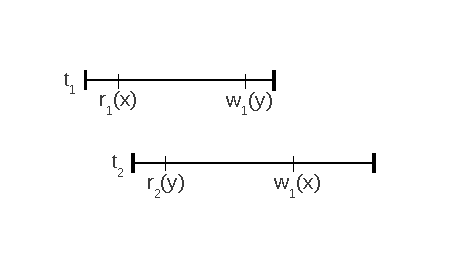
\includegraphics{images/si.pdf}
\caption{Write skew anomaly}
\label{si}
\end{figure}

\subsubsection{Multiversion Timestamp Ordering}
Multiversion timestamp ordering (MVTO) assigns each transaction a unique timestamp that is larger than that of any transaction started before it. It then maps read and write operations onto versions such that the result is equivalent to that of a serial monoversion schedule in which transactions are executed in the order of their timestamps. Operations are scheduled optimistically, so if an ordering conflict occurs that cannot be resolved, one of the transactions is forced to abort and restart.

The concrete protocol consists of the following three rules ~\cite{Weikum:2001:TIS}:
\begin{enumerate}
\item A read operation of some object $x$ by transaction $t_i$ is mapped to the latest version of $x$ written by a transaction that started before $t_i$.
\item A write operation of some object $x$ is rejected and $t_i$ aborted if a transaction that started after $t_i$ has already read a version of $x$ written by a transaction that started before $t_i$. Otherwise, it is transformed into a write operation of version $i$ on object $x$.
\item A commit operation by transaction $t_i$ is delayed until all transactions that have written versions of objects read by $t_i$ have been committed.
\end{enumerate}

MVTO prevents the write-skew anomaly through the second rule: $t_1$ is forced to abort when it attempts to write a new version of $y$, since $t_2$, which started after $t_1$ has already read the previous version. MVTO is well suited if there is little write contention and has the benefit of being deadlock free, since no locks are used and transactions only ever wait on transactions started before them to commit.

\section{Programming Model}

\subsection{Row Groups}
To enable local transactions across multiple rows, it is necessary to co-locate them in the same tablet and ensure they are not separated when the tablet that contains them is split. Since BigTable sorts tables by row key, using a common row key prefix results in rows being placed next to each other. Such a row key prefix can be a synthetic partitioning key as used in Cloud SQL Server ~\cite{Bernstein:2011:AMS:2004686.2005651} or the key of one of the rows in the group as described in Megastore ~\cite{Baker:2011:8530095}. The latter is an obvious choice if the entities stored in the rows have an inherently hierarchical relationship. We refer to rows with the same prefix as a \emph{row group} and call the prefix the \emph{group key}.

In order for the system to ensure that rows in the same row group are not split, it needs to be made aware of the group key. We do not impose restrictions on how group keys are chosen or how they are prepended as long as the resulting row key complies with the BigTable programming model. Instead, we allow users to define the mapping between row and group keys by implementing a \emph{row group policy} and associating it with the table. The system can use this function to obtain a split point that is guaranteed to be in between row groups. Note that this scheme preserves query granularity, since it allows for partial key scans as described in ~\cite{George:2011}.

Baker et al ~\cite{Baker:2011:8530095} also describe a pattern for merging multiple tables into a single table by prefixing column keys with table names. Combined with row grouping, this pattern makes it possible to co-locate rows from different tables. Note that such sparse tables are feasible in BigTable, since only cells that contain values are persisted.

\subsection{Group Transactions}
The client API includes methods for demarcating transaction boundaries using the familiar begin-commit-rollback idiom. When starting a new transaction, the client can either create a single-group or a cross-group transaction. In the former case, the transaction will abort and rollback if an operation tries to access rows outside of the group accessed by previous operations in the same transaction. In the latter case, two-phase commit is used to coordinate commits across accessed groups. This implies additional overhead and increases the risk of conflicts, so clients should use cross-group transactions sparingly. Each operation must be enlisted with the transaction before it is executed. Since Troups uses optimistic concurrency control, a transaction may abort while executing a data access or commit operation if a conflict is detected that cannot be resolved. In this case, the system rolls back any changes applied by the transaction and the client has to retry the transaction. Listing ~\ref{tran} shows how the API is used.

Troups uses the timestamp dimension to store versions created by different transactions, so timestamps are not available in the client API. This is merely the result of an implementation choice; the system could store multiple versions under a single timestamp as described in ~\cite{Peng:2010:LIP:1924943.1924961} to preserve the timestamp dimension.

\begin{lstlisting}[language=Java,caption=Group Transaction Syntax,float,label=tran,emph={begin,enlist,commit,rollback},emphstyle=\underbar]
Transaction ta = TM.begin()
try {
  Get get = new Get("1.row1")
  ta.enlist(table, get)
  table.get(get)
  Put put = new Put("1.row2")
  ta.enlist(table, put)
  table.put(put)
  ta.commit()
} catch (Transaction Aborted) {
  retry
} catch (Other Exception) {
  ta.rollback();
  exit
}
\end{lstlisting}

\subsection{Group Detection}

\section{Design}
Troups consists of three main components: a global \emph{timestamp service}, a \emph{transaction manager} that is instantiated for each tablet in the system, and a \emph{transaction client} that is associated with each BigTable client. The timestamp service generates globally unique timestamps which serve as transaction identifiers and thus allow the transaction managers to produce globally serializable schedules. It also tracks which timestamps are no longer used so that transaction managers can reclaim resources associated with those timestamps. The transaction managers implement concurrency control and recovery functionality for the tablet they are associated with. The transaction client interacts with the timestamp service and transaction managers to implement the transaction APIs.

\subsection{Timestamp Service}
The timestamp service generates globally unique timestamps that are guaranteed to be strictly increasing, but not necessarily sequential. When a client requests a new timestamp, it becomes its \emph{owner}. A timestamp is held until it is either explicitly released by the owner or implicitly released by the timestamp service. The latter happens if the timestamp service believes the owner has become unavailable, the determination of which is implementation specific. As such timestamps are transient resources. The timestamp service eventually reclaims released timestamps which are preceded by only released or reclaimed timestamps. Clients can query the value of the last reclaimed timestamp or register to be notified whenever its value changes.

To facilitate the implementation of distributed transactions, the timestamp service also allows for shared timestamp ownership through the addition of a \emph{participant} role. After an owner has acquired a timestamp, participants can acquire \emph{references} to it, which are uniquely identified for a particular timestamp. If the owner explicitly or implicitly releases the timestamp at this point, it is marked as released, so the semantics are the same as in the basic protocol. However, unlike in the basic protocol, the owner can decide to \emph{persist} a set of references. After such a call, the timestamp can only be reclaimed once all participants have explicitly released their references, even if the owner becomes unavailable. In the shared protocol clients can also inquire if a particular reference is persisted.

\subsection{Transaction Manager}
The transaction manager exposes functions to begin, commit, or abort single-group transactions for rows located its associated tablet. When begin is called, the transaction manager acquires a new timestamp from the timestamp service which it releases again when the transaction is committed or aborted. The transaction manager also exposes join, prepare, commit, and abort functions used to implement cross-group transactions. When a request is received to join an existing transaction for a specific group, it creates a new transaction branch by acquiring a reference to the existing shared timestamp. Such a transaction branch can be prepared and committed, committed in one phase, or aborted, all of which cause the transaction manager to release the timestamp reference it is holding. To enforce ACID semantics, the transaction manager intercepts all data access operations performed in the context of a transaction on the associated tablet.

\subsubsection{Concurrency Control}
Troups uses MVTO to ensure serializable transaction execution. This protocol is well suited for BigTable, because BigTable already has timestamps built into the data model and can easily provision additional storage needed for temporary versions. It is also in line with BigTable's core design principles of favoring immutability to avoid synchronization and allow for garbage collection. Since read and write operations are observed at some point before and after they are applied to the datastore, we need an extension of the basic MVTO protocol to remove the assumption that rule enforcement and data access happen as an atomic unit. We call this protocol Observer Multiversion Timestamp Ordering (OMVTO) and define it as follows.

Each read operation $r_i(x)$ of some data item $x$ by transaction $t_i$ consists of a before-read notification $br_i(x)$ and an after-read notification $ar_i(x)$. During these notifications the read operation can be transformed to and from a read operation on specific versions of $x$. This version-aware read operation is executed at some point between the two notifications. Analogously,  write operations $w_r(x)$ of data item $x$ by transaction $t_i$ consist of a before-write notification $bw_i(x)$ and an after-write notification $aw_i(x)$ with the version-aware write operation executed in between.

The OMVTO rules are as follows:
\begin{enumerate}
\item During $br_i(x)$ a read operation $r_i(x)$ is transformed into $r_i(x_k)$ where $k$ is the largest timestamp of transactions that have been scheduled to write $x$ and started before $t_i$.
\item During $ar_i(x)$, if the result set of $r_i(x_k)$ is empty, $t_i$ is aborted or forced to re-execute $r_i(x)$. Otherwise the result is returned.
\item During $bw_i(x)$ a write operation $w_i(x)$ is transformed into a write operation of $x_i$, unless a transaction $t_j$ that started after $t_i$ has already been scheduled to read $x_k$ where $k < i$. In this case $t_i$ is aborted.
\item A commit operation by transaction $t_i$ is delayed until all transactions that have written versions of objects read by $t_i$ have been committed.
\end{enumerate}

The key difference to the basic MVTO protocol is the second rule, which ensures that the result set returned by the version-aware read operation actually contains the expected version. This rule is needed, because the scheduler does not control the sequencing of the data access operations. Therefore, it is possible that a write operation is admitted, but that a read operation selected to read its version is executed before the actual write. If the reader were allowed to proceed or read an older version in this case, the timestamp ordering constraint would be violated. The correctness of the remaining rules follow from the basic MVTO protocol.

\subsubsection{Recovery}
BigTable already ensures that single row mutations are atomic. Therefore, the transaction manager only needs to ensure that all operations executed in the scope of a transaction are committed or rolled back atomically. To achieve this, the transaction manager keeps track of which cells have been written by each transaction. If a transaction is aborted, it is no longer considered for conflict detection and all transactions that read from it are aborted. Any versions written by the aborted transaction are then removed from the data store. Conversely, if a transaction is committed while transactions it read from are still active, it is blocked. If one of the writers aborts, the blocked transaction is also aborted. If all them commit, the blocked transaction is committed.

To ensure atomicity is preserved across tablet lifecycle changes and tablet server crashes, transaction state changes are logged to durable storage. These log records are indexed by group key in order to support tablet split and merge mutations. When a transaction manager is started, it replays all log records with group keys that fall into the tablets row range to reconstruct the transaction state. The transaction manager is guaranteed that all log records for any given transaction will be present, since the installed split policy prevents rows in the same row group from being split across tablets. After replaying log records, it recovers any incomplete operations. In particular, it resumes the two-phase commit process for prepared transactions with persisted timestamp references.

\subsubsection{Garbage Collection}
The transaction manager needs to periodically discard transaction state that is no longer needed to limit memory consumption and maintain efficient conflict detection. While aborted transactions can be discarded immediately, committed transactions need to be kept around for conflict detection until all transactions that precede them have committed or aborted. Since an individual transaction manager does not have a global view of which transactions are active, it relies on the timestamp manager to determine which transactions can be discarded. Ideally, all transactions with timestamps lower than the last reclaimed timestamp can be discarded, since their timestamps have been released. However, it is possible that the timestamp manager has incorrectly released timestamps that are still in use, so if an active transaction falls into this range, only transactions preceding it are discarded. The transaction manager may also receive requests to join a straggling cross-group transaction with a timestamp lower than the last discarded transaction. It must reject such requests, triggering a restart, since it no longer has all read records of later transactions needed for conflict detection.

The transaction manager must also periodically remove obselete versions from the data store and truncate the transaction log to reduce storage space. It can remove committed versions from the datastore that have been superseded by newer comitted versions if they precede the last discarded transaction. Similarly, log records can be discarded if they were created for discarded transactions.

\subsection{Transaction Client}
The transaction client forwards client-side transaction invocations to the corresponding transaction manager. For single-group transactions, it calls begin once it knows which row group is accessed by the transaction. It then associates the returned transaction identifier with each data access operation and eventually commits or aborts the transaction. If the client fails, the transaction eventually times out. For cross-group transactions, the transaction client initially obtains a shared transaction timestamp. Whenever a new row group is accessed by the transaction, it asks the corresponding transaction manager to join the transaction for the given group. Note that the same transaction manager may be asked to join the transaction for different row groups. When the transaction client receives a commit request, it either executes a single-phase commit, in case only one row group was accessed, or a two-phase commit, in case multiple row groups were accessed. In the latter case it persists the shared timestamp after all transaction managers have successfully prepared to commit their changes. At this point the transaction is guaranteed to eventually commit, even if the client fails. It then sends the commit confirmation to all transaction managers and upon receiving acknowledgements releases the shared timestamp.

By sharing the two-phase commit coordination role between the transaction client and the timestamp service, BigTable clients do not need to be made recoverable. On the other hand, the design relies on a highly available and recoverable timestamp service implementation.

\section{Implementation}
We have created a publicly available implementation of Troups\footnote{https://github.com/busjaeger/troups} based on the open source BigTable implementation HBase\footnote{http://hbase.apache.org/}. In the following sections we highlight the main implementation choices.

\subsection{Timestamp Service}
We have evaluated several implementations of the timestamp service. The first implementation is based on Zookeeper ~\cite{Hunt:2010:ZWC:1855840.1855851}, an open source implementation of the Paxos algorithm ~\cite{Lamport:1998:PP:279227.279229, Lamport:2001:PMS}. This implementation represents timestamps as ephemeral sequential nodes and shared timestamps as persistent nodes with references stored in them. Watches are used to implement notifications. Although this implementation is highly reliable, we have observed high latency for node creation. The second implementation represents timestamps as rows in an HBase table. An HBase counter is used to generate increasing timestamps. Although this implementation has shown better response times, the shared counter can become a bottleneck as the number of transactions increases. Both of these implementations are decentralized and timestamp reclamation is performed by a dedicated thread running on one of the tablet servers. To decide which tablet server should run the timestamp reclamation thread, we implemented a leader election algorithm on top of Zookeeper.

The third implementation is a centralized server more optimized for the specific protocol. It increments a persistent timestamp counter in batches and stores non-persistent timestamps in memory. The timestamp counter and persistent timestamps are stored in an HBase table, so they can be recovered if the server is restarted or crashes. However, the last reclaimed timestamp is not persisted, so if the server fails it has to assume any transactions before the first persisted timestamp are reclaimed. The benefit of this implementation is low average response time.

\subsection{Transaction Manager}
The transaction manager is implemented as a special HBase Coprocessor that exposes the transaction lifecycle operations through a Coprocessor Endpoint and intercepts HBase data access operations through the Coprocessor Observer interface.

\subsubsection{Concurrency Control}
The transaction manager implements OMVTO without explicitly tracking which versions exist in the datastore at any given time. On the before-read notification, it sets a predicate to retrieve all versions older than the transaction timestamp, instead of selecting a specific version to retrieve. On the after-read notification it then traverses the retrieved versions in descending order until it finds the first version written by a non-aborted transaction. If this version does not match the timestamp of the latest active writer of the data item that started before the reading transaction, the read is retried. Once a valid version is found, the transaction manager records the read to enable conflict detection per rule 3, and if the transaction that wrote the selected version is still active, also records a read-from relationship between the transactions to implement rule 4. Active writers are recorded during the before-write operation after enforcing rule 3. They are removed in the after-write notification once all readers that started before them have completed.

Since retrieval of aborted versions is rare, the maximum number of versions to retrieve is initially set to 1. As long as the result set contains only aborted versions, the read operation is retried with a higher maximum. The transaction manager also maintains several indices on transactions to allow for efficient conflict detection. The time complexity of enforcing the OMVTO conflict rule is $O(n \: log(m))$, where $n$ is the number of versions for the key and $m$ is the maximum number of transactions that read a given version. Therefore, the cost is relatively low if the write frequency on any given key is low.

\subsubsection{Recovery}
Removing cells for aborted transactions is done asynchronously after the transaction abort is logged. The delete operation against the datastore is idempotent so it can be retried until all cells have been successfully removed. Until this step completes, all versions written by the aborted transaction are filtered out from read result sets.

The transaction log is implemented through a dedicated HBase table with group keys serving as row keys, log sequence numbers serving as timestamps, and log records stored as values. We also attempted to store log records in the user table itself to avoid potential network overhead, however, HBase's current implementation does not allow for such callbacks from Coprocessors.

 \subsubsection{Version Cleanup}
Obsolete versions are removed from the datastore by hooking into the compaction process. To achieve this, the transaction manager returns a custom filter through the observer interface which, for each given cell, omits all versions that are smaller than the timestamp of the last discarded transaction, except for the last. This approach is more efficient than explicit deletes and was developed in ~\cite{Junqueira:2011:LTS:2056318.2057148}.

To truncate the log, the transaction manager stores the begin and end log sequence number for each transaction. Whenever it discards transaction state, it determines the highest log sequence number used by active transactions. It does this by first scanning the discarded transactions to obtain the highest begin sequence number. Since active transactions with higher timestamps may have started locally before transactions with lower timestamps, it also scans active transactions to lower the recorded log sequence number if needed. If all transactions are discarded, the highest end log sequence number is used instead. The transaction manager then deletes all log records older than the given sequence number.

\subsection{Transaction Client}
The transaction client extends the existing HBase client. It invokes transaction managers through the Coprocessor client library and propagates transaction context for enlisted data access operations by annotating them with a transaction identifier attribute. The client currently only supports a subset of HBase APIs due to time constraints.

\subsection{Row Group Detection}
The Entity Group Recommender analyzes transaction logs generated in a staging or production environment to suggest appropriate entity groupings.

The analyzer determines how data should be partitioned and where the formed partitions should be placed. We envision using a data warehouse to implement this component. The data warehouse could run on the same infrastructure to maximize utilization, or in a separate cluster to free the OLTP system from carrying the computational load. As such, possible implementation technologies include Apache Hive or a relational database system optimized for online analytical processing (OLAP). The data structures of this component will be optimized to run machine learning algorithms.

Clustering is a popular technique used in the field of machine learning to arrange similar data items together.  A specific form of clustering called hierarchical clustering involves minimizing the distance between related data items.  This would be useful in the database setting to minimize the network delay that a packet of data may experience traveling from one node to the next.  It would be especially useful in datacenters that span a wide area network where distance is indeed a major problem.  Centroid-based clustering is also useful because it finds the point within a cluster that has the shortest total distance to the other nodes.  This can be useful in determining where to place the central master node which has to communicate with all the nodes in its region.  A more general extension to this theory would involve Voronoi diagrams which arranges a diagram into multiple cells such that points in a cell are closer to each other than they are to points in other cells.

There are techniques in a subfield of machine learning called conceptual clustering in which unsupervised classification is used to create a concept description for each class. They can create a tree like clustering hierarchy which can be used to group similar data types together. It essentially creates groupings for data sets by combining the clustering and characterization phase together. It focuses on the determination of concepts to describe data. We plan to apply these different techniques and compare to see which technique can give the best results in the situations that we set up.

In particular, the clustering algorithm COBWEB is of interest. This algorithm creates a tree like structure from which each node can represent a given concept. These concepts represent sets of data that are treated as binary-valued property lists. The algorithm will take in binary values that it observes and incrementally add it into the classification tree. It will modify the tree as it goes along and perform such operations as merging concepts together, splitting concepts, adding new concepts, or adding items into a concept. We believe that this will be helpful in creating groupings for our data partitioning scheme. By arranging data into concepts, we believe that an improved partitioning scheme can be achieved.

\section{Evaluation}
In the following section we present an evaluation of our Troups implementation on HBase.

\section{Future Research}
Troups opens many opportunities for further research. To begin with, due to resource and time constraints and because there are no standardized benchmarks for BigTable transactions, we have only been able to do a limited evaluation of the current system. In future work we would like to expand the analysis and compare the system to other BigTable transaction managers.

In the area of transaction management, it would be valuable to evaluate alternative concurrency control protocols against the current MVTO implementation. Snapshot isolation or multiversion two-phase locking are plausible candidates. It would also be interesting to add support for range queries and measure the cost of partial key scans. In this context in may also make sense to allow readers to access older versions to reduce potential conflicts. Finally, different recovery strategies and version collection strategies could be compared. In particular, group commit optimizations as described in ~\cite{Weikum:2001:TIS} could be explored.

Group detection and formation can also be enhanced in several ways. Our static algorithms can be enhanced to take additional performance factors into account that arise from grouping rows. Beyond static group detection and user-defined groups lie online algorithms and automatic group formation. Such algorithms could trade off the cost of moving data with the savings of avoiding distributed transactions. They may also factor in load balancing concerns, since frequently accessed groups could heavily load certain servers. Online algorithms would be particularly well suited for applications with frequently changing access patterns. If row groups and table merging were made completely transparent to end users through a virtualized table layer, then it would be interesting to investigate for what degrees of locality it would be feasible to offer generalized ACID transactions.

\section{Conclusion}
We have described a transaction programming model and implementation for BigTable that improves data consistency without significantly impacting scalability. It achieves this by minimizing the use of distributed transactions through co-location of related data. Our approach requires no changes to BigTable or additional cluster hardware or processes. It also does not require any configuration apart from distributing the binaries throughout the cluster. Moreover, Troups can be used alongside non-transactional APIs in the same BigTable cluster.

We have also presented a flexible mechanism for forming static or dynamic row groups. We use this mechanism to co-locate rows in order to execute local transactions across them, but it can be used for many other use cases. For example, it can be used to place data groups closer to users to improve performance or to form groups in a way that better balances server load.

To aid the user in identifying which rows are frequently accessed together in transactions we have developed a clustering algorithm based on transaction logs. Users can analyze the output of this algorithm to help them in their process of deciding which rows to group together. The strength of this algorithm is TODO

Furthermore, we discussed a timestamp service that is primarily used by our transaction manager, but is generally usable in distributed systems that need to manage transient versions of data. The service is implemented as a configurable Zookeeper client, so it can be easily embedded into other applications.

Finally, we implemented a comprehensive and extensible research prototype that we plan to make publicly available to the research community through the hadoop ecosystem.


% Bibliography generation from references.bib
\bibliographystyle{IEEEtran}
\bibliography{IEEEabrv,references}

\end{document}
